\section{Roman Pot Simulation}\label{section:reconstructionSTAR_pp2pp_Sim}
\begin{figure}[h!]
	\centering
	\begin{subfigure}{.64\textwidth}
		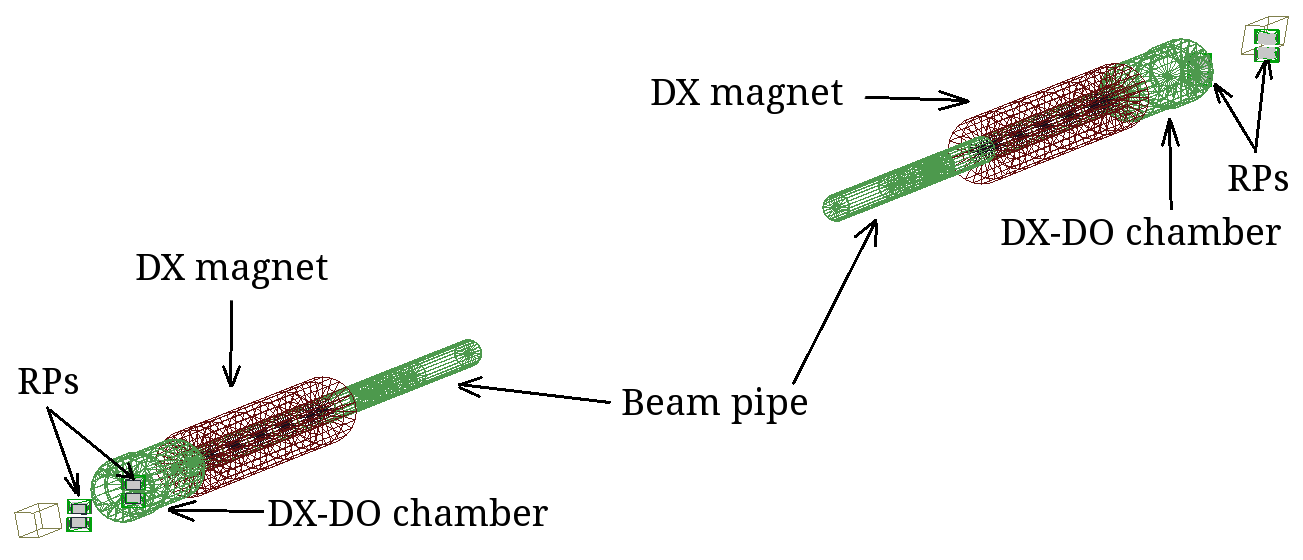
\includegraphics[width=\textwidth]{chapters/dataSampleSTAR/img/pp2ppSim/geant4plot.png}
	\end{subfigure}
	\begin{subfigure}{.34\textwidth}
		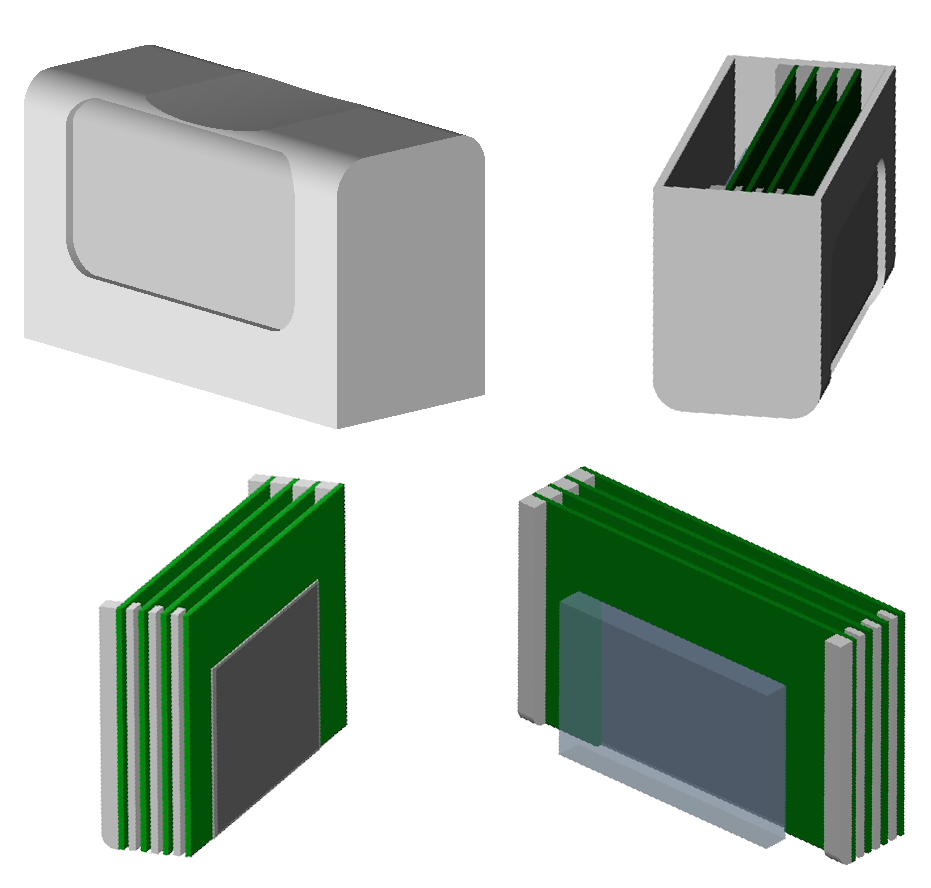
\includegraphics[width=\textwidth]{chapters/dataSampleSTAR/img/pp2ppSim/g4Rp.png}
	\end{subfigure}	
	
	\caption{(left) GEANT4 implementation of the RP system and (right) RP vessel together with SSD. Figure courtesy of R. Sikora (STAR Collaboration).}
	\label{fig:pp2ppSim}
\end{figure}

The geometry of the \ac{RP} detectors is not implemented in the~standard \ac{STAR} GEANT3 simulation. Therefore, a~standalone GEANT4 simulation of the \ac{RP} \ac{SSD} detectors~\cite{RafalInz,RafalMgr} and the \ac{RHIC} magnet lattice was developed~\cite{LukaszInz,LukaszMgr}. The application was orginally dedicated to the configuration of the \ac{RP}s for RHIC Run 2009~\cite{pp2pp:elastic}. When the \ac{RP}s were moved to their current location in the \ac{RHIC} tunnel, the simulation was updated. The geometry of  \ac{RHIC}, i.e. magnets and beampipe, is based on the technical drawings of  \ac{RHIC}, whereas the MAD-X~\cite{MADX} output provides information about the magnetic field of the RHIC DX magnets. In case of the \ac{RP} vessels and \ac{SSD}s, technical drawings together with the dedicated survey were used to best implement their geometry.

Figure~\ref{fig:pp2ppSim} shows the GEANT4 visualisation of the \ac{RP} setup together with all beam-line elements. In addition, the  implementation of the \ac{RP} vessels and \ac{SSD}s is  presented. 



 
